\chapter{temp}



\begin{figure}[htbp]
    \centering
    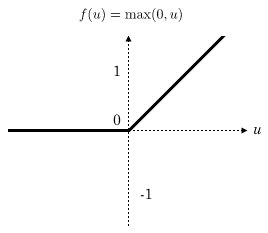
\includegraphics[width=0.7\textwidth]{Cnn1.png}
    \caption{Relu函数}
    \label{fig:Cnn1}
\end{figure}

\begin{figure}[htbp]
    \centering
    \includegraphics[width=1\textwidth]{Rnn16.png}
    \caption{cross correlation}
    \label{fig:Rnn16}
\end{figure}

\begin{figure}[!h]
    \centering
    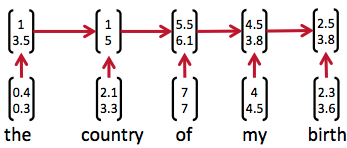
\includegraphics[width=1\textwidth]{Recu1.png}
    \caption{cross correlation}
    \label{fig:Recu1}
\end{figure}

\begin{lstlisting}[numbers=none]
    INPUT -> [[CONV]*N -> POOL?]*M -> [FC]*K
\end{lstlisting}


\begin{note}
    ???????GitHub: \url{https://github.com/hanbt/learn_dl/blob/master/rnn.py}
    (python2.7)
\end{note}


\begin{lstlisting}

\end{lstlisting}














?\ref{fig:Recu1}

??\ref{eq:Recu1}


\\\[
(.+?)\\qquad\(?(1)\)
\\\]


\begin{equation}
    \label{eq:Recu}
\end{equation}